\chapter{Introduction}

\section{Opening Thoughts}

What, exactly, is a fluid? Well, it's anything that \emph{flows}, of course. But that can mean a surprising number of things.

One obvious example is water, which we'll use extensively as our go-to fluid for a number of applications. Other fluids might be highly viscous -- syrup is a good example -- in which case the behaviour might be very different.  Later on in the book we'll take an introductory look at \emph{aerodynamics}, where the fluid is of course air.  

These are all good examples of what's called a \emph{Newtonian fluid} -- the fluid has certain, fairly simple properties and can be modelled well by a set of equations called the \emph{Navier-Stokes} equations.  Other fluids, though, are more complicated (and, for the most part, beyond the scope of this book).

For example, the behaviour of fluids with a net charge (e.g., a plasma) add interesting complications that must be dealt with by including the theory of electricity and magnetism.  Combining Maxwell's equations with the Navier-Stokes equations leads to the theory of magnetohydrodynamics, or MHD for short.

Even something as commonplace as blood, though, can be beyond the Navier-Stokes equations to model.  That's because blood is an example of a non-Newtonian fluid -- it's nonhomogeneous and is a ``shear-thinning'' fluid, which means it becomes less viscous at high shear strain.  Consider what happens to the blood during an anaphylactic shock -- an extreme allergic reaction.  The body's first response is to release histamine, which causes the blood vessels to widen.  When this happens, the blood will slow down, for reasons we'll learn have to do with conservation of mass.  But because blood is shear-thinning, it becomes more viscous as it goes slower.  This leads to a feedback loop -- increased viscosity causes the blood to slow further, causing it to be more viscous, which means the blood slows even more, and so on.  This is why anaphylaxis is so severe and needs to be treated right away with adrenaline, which increases blood flow.

As a final, surprising, example, traffic can sometimes be modelled as a fluid -- even though cars are large, discrete objects.

Although the study of fluid dynamics is centered around solving the Navier-Stokes equations, in this first chapter we'll begin with some preliminary ideas about the flow of fluids, in particular how we can mathematically describe and visualize it.  But before we start with the heavy lifting of solving differential equation, we'll also need to be able to identify various properties of the fluid, such as its vorticity and viscosity, since in many cases understanding these can lead to significantly simpler methods of solving the equations of fluid dynamics.



\section{Describing Fluid Flow}

The main goal of fluid dynamics is to find the fluid velocity $\bf{u}$ at every point $\bf{x}$ at any time $t$:
\begin{equation}
\mathbf{u} = \mathbf{u}(\mathbf{x}, t).
\end{equation}
This is a good time to discuss some of the notation we'll be using.  First, note that I'm bolding any quantity that's a \emph{vector}, like position and velocity.  Scalars are represented by italicized letters.  Secondly, I'm using $\mathbf{u}$ to denote the velocity rather than the more usual $\bf{v}$. In fact, the letter $v$ serves a different purpose -- it's the $y$ component of the fluid velocity. The $x$ and $z$ components are denoted by $u$ and $w$, respectively, so we can write the full vector form of the velocity as
\begin{equation}
\mathbf{u} = u \, \hat{i} + v \, \hat{j} + w \, \hat{k} = [u, v, w].
\end{equation}
Keep in mind that $u$, $v$, and $w$ are each functions of $x$, $y$, $z$, and time:
\[
u = u(x, y, z, t), \quad v = v(x, y, z, t), \quad \text{and} \quad w = w(x, y, z, t),
\]
and note that I'm using some vector short hand with the square brackets.

This can sometimes be confusing notation, so be careful with it.  Also note that (to add to the confusion) $u$ does double duty: it's both the $x$ component of the flow, as well as the name of the entire velocity vector field.


\begin{figure}
\centering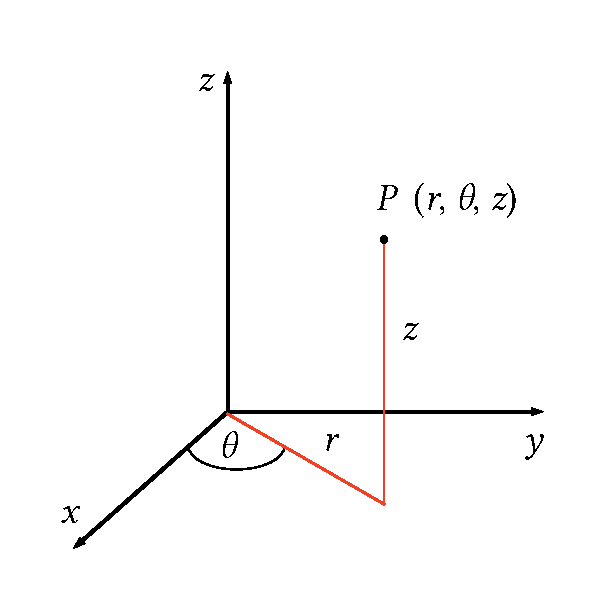
\includegraphics[width=0.5\linewidth]{Figures/Chapter1/fig_cyl_coord}
\caption{Cylindrical coordinates $(r, \theta, z)$.}
\label{fig_cyl_coord}
\end{figure}

So far, I've written everything down in Cartesian coordinates, but we'll use cylindrical coordinates $(r, \theta, z)$ frequently as well.  Figure \ref{fig_cyl_coord} shows the usual cylindrical coordinate setup (note that I'm using $\theta$ rather than the usual $\phi$; this is mostly because all my notes come from a math book), and it's clear that
\[
x = r \cos \theta, \quad y = r \sin \theta, \quad \text{and} \quad z = z.
\]
We can write the fluid velocity in cylindrical coordinates as
\begin{equation}
\label{eq_u_cyl}
\mathbf{u} = u_r(r, \theta, z, t) \hat{r} + u_\theta (r, \theta, z, t) \hat{\theta} + u_z(r, \theta, z, t) \hat{z}.
\end{equation}
I'll avoid using the ``bracket'' shorthand if we're using cylindrical coordinates, though.



In much of our examination of fluid dynamics, we'll deal with special cases and symmetries which will make our job (slightly) easier.  The below examples discuss two of these special cases.

\begin{example}[Steady Flow]
A \emph{steady flow} has no explicit time dependence, so that
\begin{equation}
\frac{\partial \mathbf{u}}{\partial t} = 0.
\end{equation}
This means that, at any point, the speed and direction of the flow are constant. We'll be dealing with this case quite frequently, especially at the beginning of the book.
\end{example}

\begin{example}[Two Dimensional Flow]
A \emph{two dimensional} flow has the form
\begin{equation}
\mathbf{u} = [u(x, y, t), v(x, y, t), 0].
\end{equation}
Note that not only is there no $z$ component to the velocity field, but there is furthermore no $z$ dependence on the
$x$ and $y$ components, either.
\end{example}





\section{Visualizing Fluid Flow}



\subsection{Vector Plots}

One way to visualize the flow of a fluid is by drawing a vector for $\mathbf{u}$ at a sample of positions and, if necessary, times.

\begin{example}[Flow about a stagnation point]
For example, consider the fluid velocity vector field
\begin{equation}
\label{eq_stag}
\mathbf{u} = [\alpha x, -\alpha y, 0].
\end{equation}
This is an example of two-dimensional, steady flow, and, as we'll see later, is the flow around a \emph{stagnation point}, which is a point in the fluid which is not flowing.  The vector plot for this flow is given in Figure \ref{fig_vector_plot}. 
\end{example}

\begin{figure}
\centering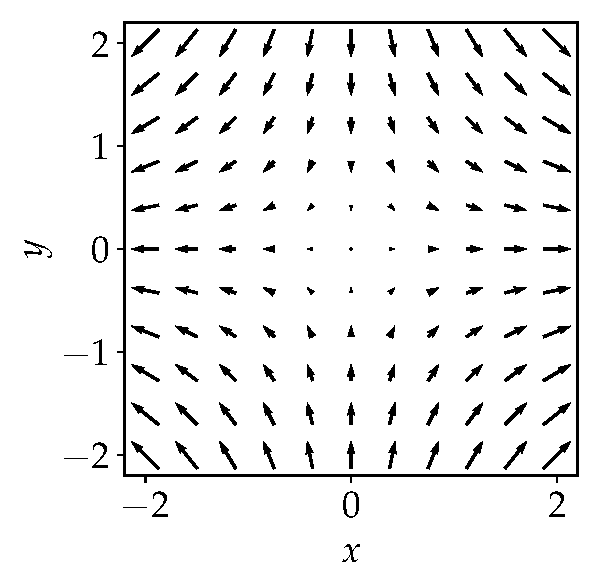
\includegraphics[width=0.5\linewidth]{Figures/Chapter1/fig_vector_plot}
\caption{A vector plot for flow about a stagnation point.  Here the parameter $\alpha = 1$.  Note that at the point $(0,0)$ the flow velocity is zero; that's what makes it a stagnation point. \href{https://nbviewer.jupyter.org/github/josephmacmillan/IntroFluidDynamics/blob/master/Jupyter/1-Introduction.ipynb\#Figure-1.2:-A-vector-plot-for-flow-about-a-stagnation-point}{[Link to Code]}}
\label{fig_vector_plot}
\end{figure}



\subsection{Streamlines}

A more common way to visualize fluids is with \emph{streamlines}.  A streamline is a curve that, at time \(t\), has the same direction as \(\mathbf{u}(\mathbf{x}, t)\) at each point. This is a concept you might be familiar with from electrodynamics -- electric field lines are very similar.  Like field lines, streamlines can't cross, since that would imply that a particular fluid element at that point would have two different velocities.  

How do we calculate (and plot) streamlines? Well, we first parameterize a streamline curve, using \(s\) as the parameter, as 
\[
x(s), \quad y(s), \quad z(s),
\] 
so that, as \(s\) changes, the functions $x$, $y$, and $z$ trace out the streamline curve.   From the definition of a streamline, we know that
\[
\frac{dx}{ds} = ku, \quad \frac{dy}{ds} = kv, \quad \frac{dz}{ds} = kw,
\] 
where \(k\) is some constant (and different streamlines will have different -- but unique -- values of \(k\)). Since \(k\) is the same along each streamline, we must have
\begin{equation}
\frac{dx/ds}{u} = \frac{dy/ds}{v} = \frac{dz/ds}{w}.
\end{equation} 
This means that, given the functional form of \(u\), \(v\), and
\(w\), we can find \(x(s)\), \(y(s)\), and \(z(s)\).

In addition to streamlines, \emph{pathlines} and \emph{streaklines} are sometimes used to visualize and describe fluid flow.  However, for steady flow -- which we'll mostly be dealing with -- they're the same as streamlines, so we won't worry about them too much.  You can watch a nice video about it (as well as some other aspects of visualizing fluids) at \url{https://youtu.be/nuQyKGuXJOs}\footnote{This is just one video in a whole series by the National Committee for Fluid Mechanics Films.  Despite their age, they're great, and I highly recommend watching the ones that are relevant to us.}, and Problem \ref{prob_unsteady} takes a look at an unsteady case where the path lines are different from the streamlines.

\begin{example}[Plotting Streamlines]
As an example of calculating and then plotting streamlines, let's go back to our flow about a stagnation point, Equation \ref{eq_stag}.  Since this is two dimensional flow, we can ignore $w$ and $z$ dependence and look at 
\[
\frac{dx/ds}{u} = \frac{dy/ds}{v}.
\]
Plugging in \(u\) and \(v\) for this case, and removing the parameter $s$ for simplicity, gives us
\[
\frac{dx}{\alpha x} = -\frac{dy}{\alpha y}.
\] 
Integrating both sides and solving for \(y\) gives the function 
\begin{equation}
y(x) = \frac{c}{x}.
\label{eq_stream_ex}
\end{equation}
That's our answer; \(c\) is the integration constant, which will vary from streamline to streamline.  Figure \ref{fig_streamline_example} shows the streamlines plotted; as usual, code to do this is provided separately.
\end{example}

\begin{figure}[t]
\centering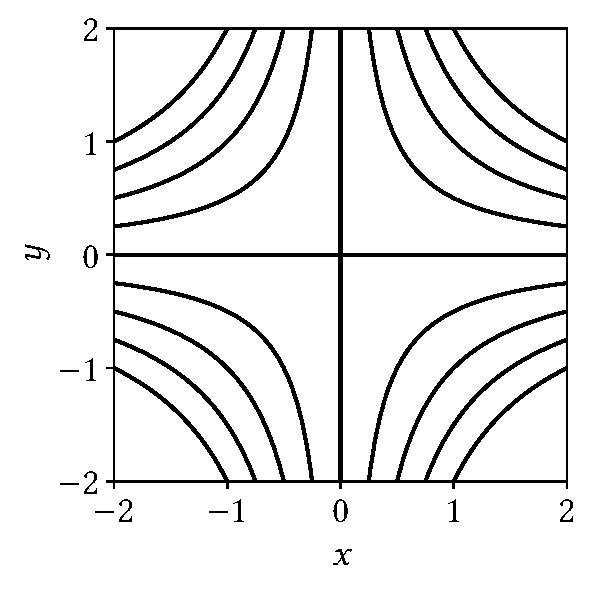
\includegraphics[width=0.5\linewidth]{Figures/Chapter1/fig_streamline_example}
\caption{Streamlines plotted from Equation \ref{eq_stream_ex}, for a variety of values of $c$ ranging from $-2$ to $2$.  Note that the streamlines cross at the stagnation point; that's the only place where they're allowed to. \href{https://nbviewer.jupyter.org/github/josephmacmillan/IntroFluidDynamics/blob/master/Jupyter/1-Introduction.ipynb\#Figure-1.3:-Plotting-Streamlines}{[Link to code]}}
\label{fig_streamline_example}
\end{figure}







\section{Total Derivative and Acceleration}

Now that we know how to visualize the flow of a fluid, we need to be able to calculate how it \emph{changes}.  

Let $f(x, y, z, t)$ be some quantity of interest -- it might be a component of velocity ($u$ or $v$, say), or maybe the density of the fluid $\rho$, or even the concentration $c$ of a certain pollutant in the fluid.  If we're then looking at one particular (fixed) location -- say, $x, y, z$ -- in the fluid, then $\partial f / \partial t$ gives the rate of change of $f$ at that position.

On the other hand, we might want to know how $f$ changes as we move along with the fluid.  In this case, we might imagine attaching ourselves to a certain \emph{fluid element} -- a small ``blob'' of the fluid -- and measuring how $f$ changes as we move along with it.  This rate of change is given by the so-called \emph{total} or \emph{material} derivative,\footnote{There are many other names for this kind of derivative, too; according to Wolfram MathWorld, it's also called the convective derivative, the advective derivative, derivative following the motion, hydrodynamic derivative, and Lagrangian derivative, among a few others.}
\[
\frac{Df}{Dt} \equiv \frac{df}{dt} = \frac{d}{dt} f[x(t), y(t), z(t), t].
\]
Now, $x(t)$, $y(t)$, and $z(t)$ all change as we move with the flow, and of course
\[
\frac{dx}{dt} = u, \quad \frac{dy}{dt} = v, \quad \text{and} \quad \frac{dz}{dt} = w.
\]
So, applying the chain rule to the derivative above, we get
\begin{align*}
\frac{Df}{Dt} & =  \frac{\partial f}{\partial x}\frac{dx}{dt} + \frac{\partial f}{\partial y}\frac{dy}{dt} + \frac{\partial f}{\partial z}\frac{dz}{dt} + \frac{\partial f}{\partial t} \\
& = u \frac{\partial f}{\partial x} + v \frac{\partial f}{\partial y} + w \frac{\partial f}{\partial z} + \frac{\partial f}{\partial t}.
\end{align*}
This can be written more compactly using vectors:
\begin{equation}
\label{eq_total_deriv}
\boxed{
\frac{Df}{Dt} = \frac{\partial f}{\partial t} + (\mathbf{u} \cdot \boldsymbol{\nabla}) f.
}
\end{equation}
Careful with that dot product; the gradient operator $\boldsymbol{\nabla}$ operates on the function $f$, so you can't switch the order.  In this case, $(\mathbf{u} \cdot \boldsymbol{\nabla}) \neq (\boldsymbol{\nabla} \cdot \mathbf{u})$.

As an example of applying the total derivative, let's take $f$ to be the fluid velocity itself:
\begin{equation}
\label{eq_accel}
\boxed{
\frac{D\mathbf{u}}{Dt} = \frac{\partial \mathbf{u}}{\partial t} + (\mathbf{u} \cdot \boldsymbol{\nabla}) \mathbf{u}.
}
\end{equation}
This, as you might suspect, is the \emph{acceleration} of the fluid element at position $\mathbf{x}$.

Note that if the material derivative is \emph{zero},
\[
\frac{Df}{Dt} = 0,
\]
that implies that the quantity $f$ doesn't change \emph{for a particular fluid element.}  On the other hand, if just
\[
(\mathbf{u} \cdot \boldsymbol{\nabla}) f = 0,
\]
that means that $f$ will be constant \emph{along a streamline.}  This isn't obvious (at least to me), so let's prove it.  Let $\hat{\mathbf{e}}_s$ be a unit vector that is always parallel to a streamline in the direction of the flow.  Since a streamline is always tangent to the flow, we can write
\[
\mathbf{u} = |\mathbf{u}| \, \hat{\mathbf{e}}_s,
\]
so that
\[
(\mathbf{u} \cdot \boldsymbol{\nabla}) f = (|\mathbf{u}| \, \hat{\mathbf{e}}_s \cdot \boldsymbol{\nabla}) f = (|\mathbf{u}| \frac{\partial }{\partial s} )f = |\mathbf{u}| \frac{\partial f}{\partial s} = 0.
\]
Thus $\partial f / \partial s = 0$ and the quantity $f$ must be constant along the direction $s$, which is along the streamline.

\begin{example}[Acceleration of the fluid]
Let's return to our flow around a stagnation point.  What is the acceleration of the flow?

Well, clearly $\partial \mathbf{u} /\partial t = 0$ (the flow is steady), and so
\[
\frac{D \mathbf{u}}{Dt} = (\mathbf{u} \cdot \boldsymbol{\nabla} ) \mathbf{u} = \left( u \frac{\partial}{\partial x} + v\frac{\partial}{\partial y} \right) \mathbf{u}.
\]
At this point is probably easiest to work out each vector component separately:
\[
\frac{D u}{Dt} =  u \frac{\partial u}{\partial x} + v\frac{\partial u}{\partial y}  = \alpha^2 x,
\]
and
\[
\frac{D v}{Dt} =  u \frac{\partial v}{\partial x} + v\frac{\partial v}{\partial y}  = \alpha^2 y.
\]
So the acceleration is
\[
\frac{D \mathbf{u}}{Dt} = \alpha^2 x \, \hat{i} + \alpha^2 y \, \hat{j} = [\alpha^2 x, \alpha^2 y].
\]

\end{example}




\section{Incompressible and Irrotational Flow}

\subsection{The Incompressibility Condition}
\label{sec_incompressibility}

Except in one notable case -- gas dynamics -- we'll be dealing with fluids that are \emph{incompressible}.  This essentially just means that the density of the fluid is constant under pressure -- you can't compress it; stated another way, it means that a ``dyed'' blob of fluid can't change in volume as it moves.  Water is a good example of an incompressible fluid, and we'll even treat air as incompressible in some cases.

We need to be able to write down a mathematical statement of incompressibility.  To do this, consider a fixed, closed surface $S$ in the fluid.  By ``fixed,'' I mean that it's fixed in space, so fluid can move into this closed volume $V$ at some places and out at others; if the fluid is incompressible, though, then however much fluid is \emph{entering} the region must equal the amount that is \emph{leaving}.  

\begin{figure}
\centering
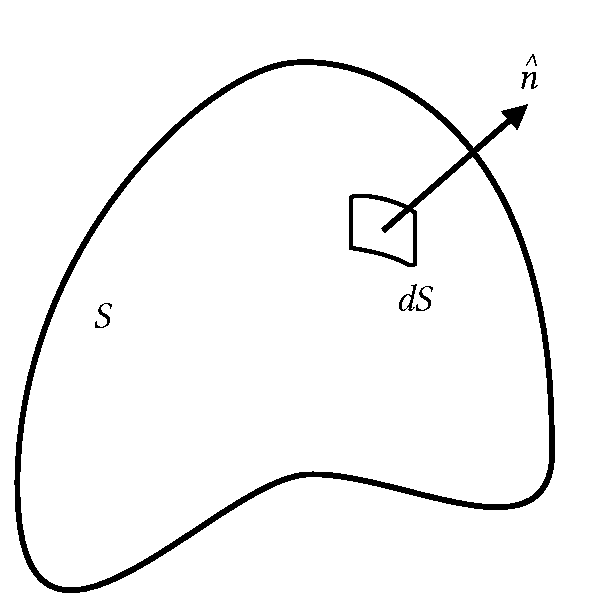
\includegraphics[width=0.5\linewidth]{Figures/Chapter1/fig_closed_surface}
\caption{A fixed, close surface.}
\label{fig_closed_surface}
\end{figure}

Consider, then, an infinitesimally small piece of $S$ -- call it $dS$ (see Figure \ref{fig_closed_surface}).  The amount of fluid that is leaving $V$ through $dS$ is given by
\[
\mathbf{u} \cdot \hat{n} \, dS.
\]
This expression, where $\mathbf{u}$ is the fluid velocity at the location of $dS$ and $\hat{n}$ points normal to the surface $dS$ but in the outward direction, is a \emph{volume flow rate}.  It measures the volume of fluid that passes through $dS$ per unit time.  The dot product ensureS we get only that fluid which is moving \emph{through} the tiny surface, whether it's flowing outward (positive dot product) or inward (negative dot product).

To find the total amount of fluid leaving the entire surface $S$, we can just integrate over that surface:
\[
\int_S \mathbf{u} \cdot \hat{n} \, dS
\]
is the net volume rate at which fluid is leaving.  However, for an incompressible fluid, we know this must be \emph{zero}.

To write this in a form a little more usable, we can apply the divergence theorem (you remember that from vector calculus, right?),
\[
\int_S \mathbf{F} \cdot \hat{n} \, dS = \int_V \boldsymbol{\nabla} \cdot \mathbf{F} \, dV,
\]
where $\mathbf{F}$ is some general vector field.  Our incompressibility condition then becomes
\[
\int_V \boldsymbol{\nabla} \cdot \mathbf{u} \, dV = 0.
\]
However, this must be true \emph{anywhere} in the fluid and for any size volume; that means the integrand itself must be zero:
\begin{equation}
\label{eq_incompressibility}
\boxed{
\boldsymbol{\nabla} \cdot \mathbf{u} = 0.
}
\end{equation}
This is the \emph{incompressibility condition}; unless we say otherwise, every flow must obey it.

\begin{example}[Incompressible flow]
Is our flow about a stagnation point incompressible?  Let's check.  Recall that $\uu = [\alpha x, -\alpha y]$.  The divergence of $\mathbf{u}$ is then
\[
\div \uu = \frac{\partial u}{\partial x} + \frac{\partial v}{\partial y} = \alpha + (-\alpha) = 0,
\]
just as we require.
\end{example}


\subsection{Vorticity}

The \emph{vorticity} of a flow is defined as
\begin{equation}
\boldsymbol{\omega} = \boldsymbol{\nabla} \times \mathbf{u}.
\end{equation}
For a two dimensional flow $\uu = [u(x, y), v(x, y), 0]$, we can write the vorticity as $\boldsymbol{\omega} = [0,0,\omega]$, where
\[
\omega = \frac{\partial v}{\partial x} - \frac{\partial u}{\partial y}
\]
(note the difference between the bolded $\boldsymbol{\omega}$ and the non-bold $\omega$ -- one is the full vector, and one is just the magnitude of that vector).

What, exactly, is vorticity?  It's related to the \emph{rotation} of the flow, but is a little trickier than that.  A couple of examples is probably best first.

\begin{example}[Vorticity of shear flow]
The flow given by $\uu = [\beta y, 0, 0]$ is called a \emph{shear flow}; a vector plot is shown in Figure \ref{fig_shear}.  This fluid is clearly \emph{not} rotating, but it does have vorticity.  Since it's two dimensional, we can easily calculate $\omega$:
\[
\omega = \frac{\partial v}{\partial x} - \frac{\partial u}{\partial y} = -\beta.
\]
\end{example}

\begin{figure}
\centering
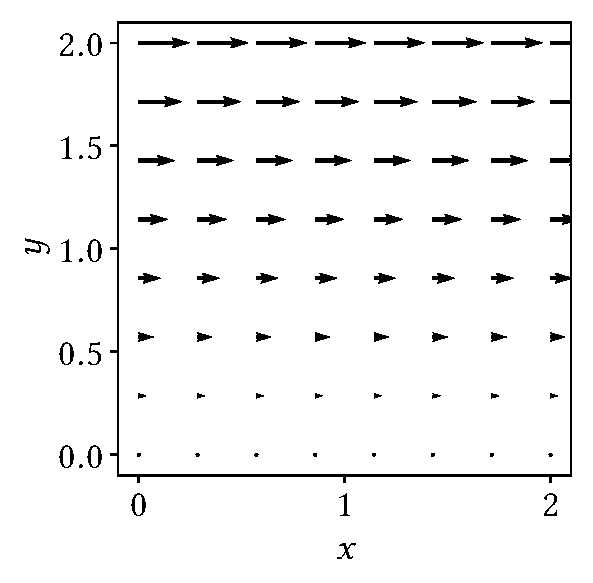
\includegraphics[width=0.5\linewidth]{Figures/Chapter1/fig_shear_vector}
\caption{A shear flow, with $\beta = 1$.  \href{https://nbviewer.jupyter.org/github/josephmacmillan/IntroFluidDynamics/blob/master/Jupyter/1-Introduction.ipynb\#Figure-1.6:-A-shear-flow}{[Link to code]}}
\label{fig_shear}
\end{figure}

\begin{example}[Vorticity of line vortex]
\label{ex_vorticity_line_vortex}
Next, let's look at the flow
\begin{equation}
\uu = \frac{k}{r} \, \hat{\theta}.
\end{equation}
This is written in cylindrical coordinates, and the vector plot is shown in Figure \ref{fig_vortex}.  We'll be seeing this kind of flow quite a bit, so make sure you're familiar with it -- but for now all we need to know is that the fluid is clearly rotating.  Despite this, the vorticity is actually zero; I'll let you show this for homework (see Problem \ref{prob_vortex_vorticity}).
\end{example}

\begin{figure}
\centering
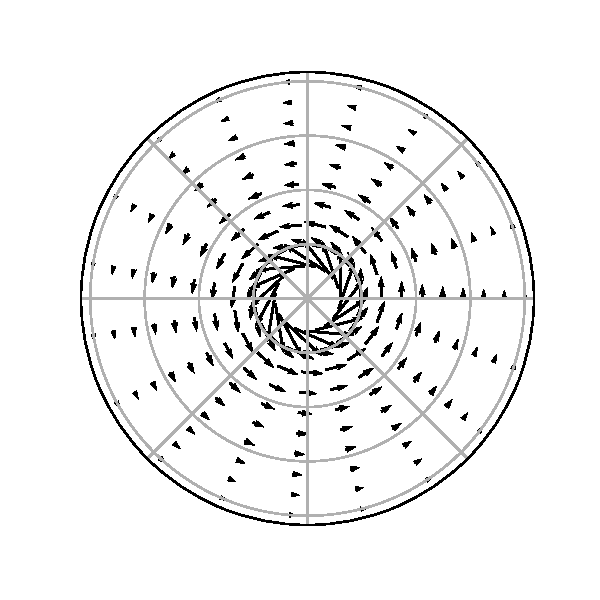
\includegraphics[width=0.5\linewidth]{Figures/Chapter1/fig_line_vortex_vector}
\caption{A line vortex flow, with $k = 1$. \href{https://nbviewer.jupyter.org/github/josephmacmillan/IntroFluidDynamics/blob/master/Jupyter/1-Introduction.ipynb\#Figure-1.6:--Line-vortex}{[Link to code]}}
\label{fig_vortex}
\end{figure}

Despite these examples, vorticity really is related to the rotation of the flow -- but it's the \emph{local} rotation that it measures.  If we built a ``vorticity meter,'' using two pieces of plastic and marking one tip so we can see it, the difference between a globally rotating flow and the line vortex example is very noticeable; see Figure \ref{fig_vorticity_meter}.

\begin{figure}
\centering
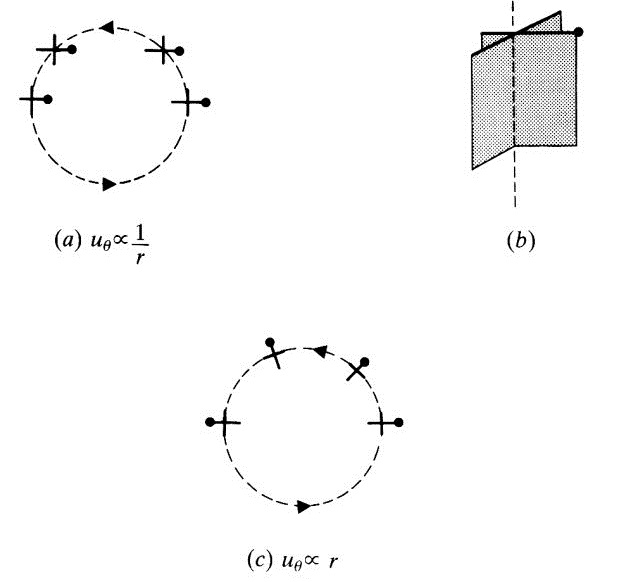
\includegraphics[width=0.7\linewidth]{Figures/Chapter1/fig_vorticity_meter.jpg}
\caption{A simple vorticity meter shows the difference between two rotating flows; it measures the \emph{local} rotation in a fluid. (Figure from \emph{Elementary Fluid Dynamics} by D. J. Acheson.) }
\label{fig_vorticity_meter}
\end{figure}

Finally, a bit of terminology: if the vorticity of a flow is zero, we say that it is \emph{irrotational}, so that
\begin{equation}
\boxed{
\boldsymbol{\nabla} \times \mathbf{u} = 0
}
\end{equation}
for an irrotational flow.





\section{Viscosity}
\label{sec_viscosity}

Experiment shows that a fluid doesn't ``slip'' along a boundary; instead, there is a thin boundary layer across which the flow speed drops smoothly and rapidly to zero (see Figure \ref{fig_boundary}).  The fluid elements in contact with the surface therefore move with the surface; this is called the \emph{no-slip condition}.

\begin{figure}
\centering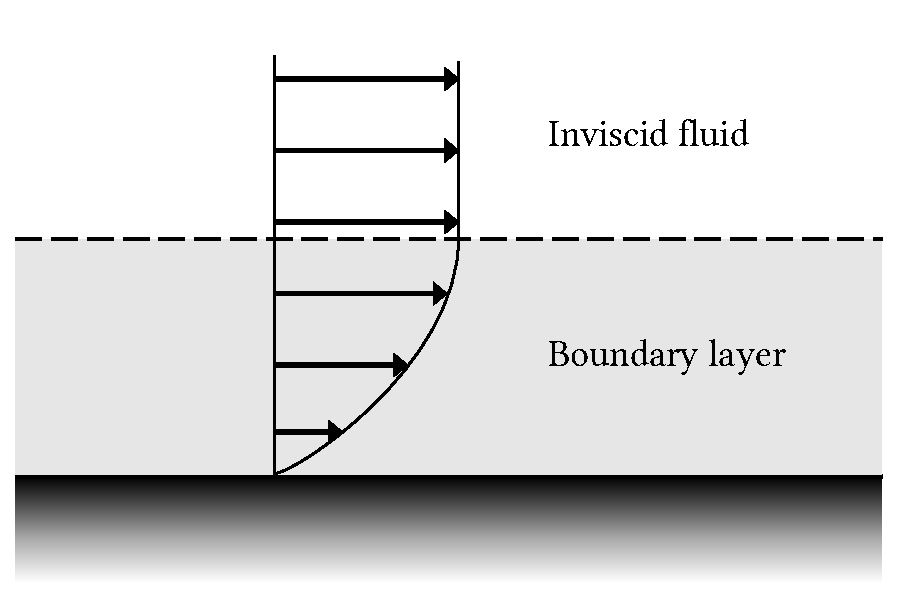
\includegraphics[width=0.7\linewidth]{Figures/Chapter1/fig_boundary_layer}
\caption{The boundary layer in a viscous fluid.  The arrow here represent the fluid velocity in the horizontal direction -- above the boundary layer, we can treat the fluid as inviscid, but within the velocity drops off to zero.}
\label{fig_boundary}
\end{figure}

The boundary layer comes from the viscosity of the fluid, which is defined (for so-called Newtonian fluids) via the tangential stress $\tau$,
\begin{equation}
\label{eq_visc_def}
\tau = \mu \frac{du}{dy}.
\end{equation}
We'll see where this comes from later on; for now, the quantity we want to focus on is the \emph{coefficient of viscosity} $\mu$.

Actually, we'll more frequently use the \emph{kinematic viscosity} $\nu$, defined by
$$
\nu \equiv \frac{\mu}{\rho},
$$
where $\rho$ is the density of the fluid. Some common viscosities (for a temperature of $15^\circ$C) are shown in Table \ref{tab_viscosity}.

\begin{table}[t]
\centering
  \begin{tabular}{l|l}
  & $\nu$ (cm$^2$/s) \\
  \hline \\
  Water & 0.01 \\
  Air & 0.15 \\
  Olive oil & 1.0 \\
  Glycerine & 18 \\
  Golden syrup & 1200
  \end{tabular}
  \caption{The viscosity of some fluids.}
  \label{tab_viscosity}
\end{table}

In some situations, the viscosity of a fluid can be neglected; we'll call the fluid \emph{inviscid} in that case:
\begin{equation}
\boxed{
\nu = 0
}
\end{equation}
for inviscid flow.  Even in situations where the viscosity is very small, though, the presence of the boundary layer can add significant complexity.  Because of the much larger velocity gradient within the boundary layer (where the fluid speed drops to zero  rapidly), the viscous stress becomes significant there, even when $\mu$ is normally small enough that we could neglect viscous effects elsewhere in the flow.

There's an additional feature of boundary layers that make them important dynamically -- in certain situations, they can actually separate from the boundary itself, causing the \emph{entire} flow to be quite different than that predicted by inviscid theory.  This is shown in Figure \ref{fig_boundary_sep} for low-viscosity flow past a cylinder.  Inviscid theory predicts the flow to the left, but boundary layer separation causes the flow on the right, where a large wake has developed past the cylinder.

\begin{figure}[t]
\centering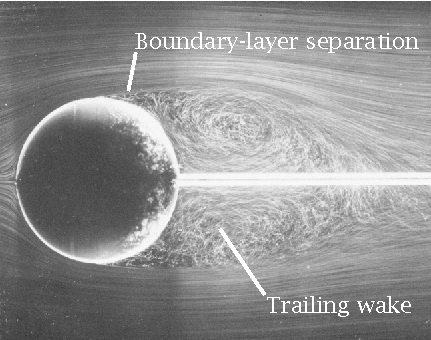
\includegraphics[width=0.5\linewidth]{Figures/Chapter1/fig_boundary_layer_sep.png}
\caption{Boundary layer separation occurring in flow past a smooth sphere.  (Photo adapted from \emph{An Album of Fluid Motion} by Milton Van Dyke.) }
\label{fig_boundary_sep}
\end{figure}

One way to characterize how important viscosity is to the flow dynamics is with the Reynolds number, defined by
\begin{equation}
R = \frac{UL}{\nu},
\end{equation}
where $U$ and $L$ are velocity and length scales characteristic to the flow (say, for example, the speed of an airplane and the width of its wing).  For large Reynolds number -- greater than a few thousand -- viscosity can be neglected, and the flow can become unstable and \emph{turbulent}.  Below this the flow is smooth, or \emph{laminar}, but viscosity effects can still usually be neglected.  For small Reynolds number, however -- less than one -- viscosity becomes important in how the fluid behaves.









\section*{Problems}
\addcontentsline{toc}{section}{Problems}

\begin{problem}[Streamlines]
Consider the flow given by 
\[
\uu = [x, x(x-1)(y+1), 0].
\]
Find an equation for the streamlines of the flow and plot them.
\end{problem}

\begin{problem}[ Unsteady flow]
\label{prob_unsteady}
Consider the \emph{unsteady} flow given by
\[
\mathbf{u} = [U, kt],
\]
where $U$ and $k$ are constants.  Show that the streamlines are straight lines at any particular point in time, and describe their behaviour as time goes on.  Then show that the path a fluid particle follows is parabolic rather than a straight line.  This is an example of how, for unsteady flow, fluid elements do not follow streamlines.

\end{problem}

\begin{problem}[Vector calculus practice]

Calculate the divergence and curl of the following vector fields.  State which flows are incompressible and which are irrotational (or both).

\begin{align*}
\text{(a) } & \mathbf{u} = [x^2, 3xz^2, -2xz] \\
\text{(b) } & \mathbf{u} = [xy, 2yz, 3zx] \\
\text{(c) } & \mathbf{u} = [y^2, 2xy+z^2, 2yz].
\end{align*}

\end{problem}

\begin{problem}[More vector calculus practice]
\label{prob_vc2}
Prove that the curl of a gradient  is always zero and that the divergence of a curl is always zero.

\end{problem}


\begin{problem}[Concentration of a pollutant]
Consider the flow about a stagnation point,
\[
\mathbf{u} = [\alpha x, -\alpha y],
\]
where $\alpha$ is a positive constant.  Suppose a pollutant is introduced into the fluid, and it's concentration is given by
\[
c(x, y, t) = \beta x^2 y e^{-\alpha t},
\]
for $y>0$, and where $\beta$ is a constant.  Does the pollutant concentration for any particular fluid element change with time?
\end{problem}

\begin{problem}[Acceleration of a rotating fluid]
A fluid in uniform rotation with angular velocity $\Omega$ is given by
\[
\uu = [-\Omega y, \Omega x, 0].
\]
Calculate the acceleration of the fluid and show that it can be written as
\[
-\Omega^2 \mathbf{r}.
\]
Is this acceleration what you expect?  Why or why not?
\end{problem}


\begin{problem}[Conservation of mass]
If the fluid is compressible, we can derive a condition to replace Equation \ref{eq_incompressibility} by assuming that mass must be conserved.  Use arguments similar to those in Section \ref{sec_incompressibility} to show that it implies
\begin{equation}
\frac{\partial \rho}{\partial t} + \div (\rho \uu ) = 0.
\end{equation}
Show also that, if the density is constant in space and time, this reduces to the usual incompressibility condition.
\end{problem}


\begin{problem}[Vorticity of a line vortex]
\label{prob_vortex_vorticity}
Show that the vorticity of a line vortex, 
\[
\uu = \frac{k}{r} \hat{\theta},
\]
is zero everywhere except at the origin, where it blows up.
\end{problem}



\begin{problem}[The Reynolds number]

Give an order of magnitude estimate of the Reynolds number for

(a) Flow past the wing of a Boeing 737 cruising at 150 m/s.

(b) A thick layer of golden syrup draining off a spoon.

(c) Air flowing through the trachea during normal breathing.

(d) Water flowing through a creek bed.

You'll have to estimate a speed and size for most of these.  Which could be turbulent?  Which would require viscous flow theory, and which inviscid theory?

\end{problem}
